\documentclass[11pt,a4paper]{article}

% ===== PACKAGES =====
\usepackage[utf8]{inputenc}
\usepackage[T1]{fontenc}
\usepackage[english]{babel}
\usepackage{geometry}
\usepackage{graphicx}
\usepackage{amsmath}
\usepackage{amssymb}
\usepackage{booktabs}
\usepackage{hyperref}
\usepackage{listings}
\usepackage{xcolor}
\usepackage{float}
\usepackage{caption}
\usepackage{subcaption}
\usepackage{tikz}
\usepackage{fancyhdr}
\usepackage{titlesec}
\usepackage{enumitem}
\usepackage{microtype}
\usepackage{parskip}
\usepackage{colortbl}
\usepackage{array}
\usepackage{tcolorbox}
\tcbuselibrary{skins,breakable}

\usetikzlibrary{shapes,arrows,positioning,shadows,calc,backgrounds}

% ===== COLOR PALETTE =====
\definecolor{primary}{HTML}{1E3A5F}        % Deep navy blue
\definecolor{secondary}{HTML}{2B7A78}      % Teal accent
\definecolor{lightbg}{HTML}{F8FAFC}        % Light gray
\definecolor{textdark}{HTML}{1E293B}       % Dark text
\definecolor{textmuted}{HTML}{64748B}      % Muted text
\definecolor{codebg}{HTML}{F1F5F9}         % Light code background

% ===== PAGE GEOMETRY =====
\geometry{
    top=2.5cm,
    bottom=2.5cm,
    left=2.5cm,
    right=2.5cm,
    headheight=22pt
}

% ===== FANCY HEADER/FOOTER =====
\pagestyle{fancy}
\fancyhf{}
\fancyhead[L]{\small\color{textmuted}\nouppercase{\leftmark}}
\fancyhead[R]{\small\color{textmuted}\thepage}
\fancyfoot{}
\renewcommand{\headrulewidth}{0.4pt}
\renewcommand{\headrule}{\hbox to\headwidth{\color{secondary}\leaders\hrule height \headrulewidth\hfill}}

% ===== SECTION STYLING =====
\titleformat{\section}
    {\Large\bfseries\color{primary}}
    {\thesection}
    {0.8em}
    {}

\titleformat{\subsection}
    {\large\bfseries\color{primary}}
    {\thesubsection}
    {0.5em}
    {}

\titleformat{\subsubsection}
    {\normalsize\bfseries\color{textdark}}
    {\thesubsubsection}
    {0.5em}
    {}

% ===== HYPERREF SETUP =====
\hypersetup{
    colorlinks=true,
    linkcolor=primary,
    filecolor=primary,
    urlcolor=secondary,
    citecolor=primary,
}

% ===== CODE LISTINGS STYLE =====
\lstset{
    backgroundcolor=\color{codebg},
    basicstyle=\ttfamily\small,
    breaklines=true,
    captionpos=b,
    commentstyle=\color{textmuted},
    keywordstyle=\color{primary}\bfseries,
    stringstyle=\color{secondary},
    frame=single,
    framerule=0.5pt,
    rulecolor=\color{textmuted!50},
    numbers=left,
    numberstyle=\tiny\color{textmuted},
    tabsize=2,
    xleftmargin=1.5em,
    framexleftmargin=1.5em,
    aboveskip=1em,
    belowskip=1em,
}

% ===== TCOLORBOX STYLES =====
\newtcolorbox{highlightbox}[1][]{
    enhanced,
    colback=lightbg,
    colframe=secondary,
    leftrule=3pt,
    rightrule=3pt,
    toprule=3pt,
    bottomrule=3pt,
    arc=2mm,
    boxsep=5pt,
    left=8pt,
    fonttitle=\bfseries\color{primary},
    title=#1,
}

\newtcolorbox{mathbox}{
    enhanced,
    colback=lightbg,
    colframe=secondary,
    boxrule=0.5pt,
    arc=2mm,
    boxsep=8pt,
}

% ===== CUSTOM COMMANDS =====
\newcommand{\keyword}[1]{\textcolor{primary}{\textbf{#1}}}

% ===== TABLE STYLING =====
\newcolumntype{L}[1]{>{\raggedright\arraybackslash}p{#1}}

% ===== DOCUMENT BEGINS =====
\begin{document}

% ===== TITLE PAGE =====
\thispagestyle{empty}

\vspace*{3cm}

\begin{center}
    {\small\textsc{Master 2 Data Science -- Institut Polytechnique de Paris}}
    
    \vspace{0.2cm}
    
    {\small\textsc{Data Stream Processing}}
    
    \vspace{3cm}
    
    {\fontsize{32}{36}\selectfont\textbf{StormWatch AI}}
    
    \vspace{0.5cm}
    
    {\large A Real-Time Weather Advisory System}
    
    \vspace{0.3cm}
        
    \vspace{4cm}
    
    {\large\textbf{Nardi Xhepi}}
    
    {\small\texttt{nardi.xhepi@polytechnique.edu}}
    
    \vspace{0.5cm}
    
    {\large\textbf{Augustin Bresset}}
    
    {\small\texttt{augustin.bresset@ip-paris.fr}}
    
    \vspace{4cm}
    
    {\large December 2025}
    
\end{center}

\newpage

% ===== ABSTRACT =====
\thispagestyle{empty}
\vspace*{1.5cm}

\begin{center}
    {\Large\color{primary}\textbf{Abstract}}
\end{center}

\vspace{0.8cm}

\noindent
Modern weather applications increasingly demand intelligent, conversational interfaces capable of answering complex natural language queries about atmospheric conditions. This report presents \textbf{StormWatch AI}, a real-time weather advisory system that integrates Apache Kafka for stream processing, Qdrant vector database for semantic storage, and a Retrieval-Augmented Generation (RAG) pipeline for intelligent query answering.

\vspace{0.5em}

\noindent
The system ingests weather data from the OpenWeatherMap API and French weather news from Le Monde RSS feeds, processes them through a distributed streaming architecture, generates semantic embeddings using sentence transformers, and provides natural language responses via Groq's LLM inference API.

\noindent
The project can be found on GitHub at \url{https://github.com/nardi-xhepi/stormwatch-ai}.

\vspace{1em}

\begin{highlightbox}[Key Features]
\begin{itemize}[leftmargin=1.5em, itemsep=0.2em, topsep=0.3em]
    \item Real-time weather data streaming with automatic API fallback
    \item Type-specific retrieval strategies for structured and unstructured data
    \item Natural language interface for weather queries and advisories
\end{itemize}
\end{highlightbox}


\newpage

% ===== TABLE OF CONTENTS =====
\tableofcontents
\newpage

%% ========================================
\section{Introduction}
%% ========================================

Weather information plays a critical role in daily decision-making, influencing activities ranging from transportation planning to agricultural operations. Traditional weather applications provide static displays of meteorological data (temperature, humidity, wind speed), but contemporary users increasingly expect more sophisticated interfaces. They want to ask natural language questions like \textit{``Is it safe to drive today?''} or \textit{``Should I bring an umbrella?''} and receive contextual, actionable insights rather than raw data.

The emergence of large language models (LLMs) and vector databases has created new opportunities for building conversational weather systems. However, integrating these technologies with real-time data streams presents significant architectural challenges. Weather data must flow continuously from external APIs, undergo processing and semantic encoding, and remain available for rapid retrieval during query processing. The system must handle the inherent tension between data freshness and query latency.

Our project addresses these challenges through \textbf{StormWatch AI}, a system that unifies three technological paradigms:

\begin{enumerate}[leftmargin=2em, itemsep=0.3em]
    \item \textbf{Stream Processing} via Apache Kafka ensures continuous data freshness with fault-tolerant message delivery
    \item \textbf{Vector Databases} enable semantic similarity search across weather observations
    \item \textbf{Retrieval-Augmented Generation} provides intelligent responses grounded in current conditions
\end{enumerate}


\newpage
%% ========================================
\section{External Services and Data Sources}
%% ========================================

StormWatch AI integrates with two external cloud services: \textbf{OpenWeatherMap} for meteorological data and \textbf{Groq} for natural language generation.

\subsection{Weather Data: OpenWeatherMap API}

OpenWeatherMap~\cite{openweather} is a widely-used weather data provider offering global coverage through a RESTful API. The free tier provides access to several endpoints:

\begin{table}[H]
\centering
\caption{OpenWeatherMap API Endpoints}
\renewcommand{\arraystretch}{1.3}
\begin{tabular}{l l p{6cm}}
\toprule
\textbf{Endpoint} & \textbf{URL} & \textbf{Description} \\
\midrule
One Call 3.0 & \texttt{/data/3.0/onecall} & Primary: current, forecast, alerts (rate-limited) \\
Current Weather & \texttt{/data/2.5/weather} & Fallback: real-time observations \\
5-Day Forecast & \texttt{/data/2.5/forecast} & Fallback: 3-hour interval predictions \\
Air Quality & \texttt{/data/2.5/air\_pollution} & Always used: PM2.5, PM10, AQI (separate quota) \\
\bottomrule
\end{tabular}
\end{table}

The system primarily uses the One Call 3.0 API which bundles current weather, forecasts, and alerts in a single request. When rate limits are exceeded, the producer automatically falls back to the legacy 2.5 API endpoints for current conditions and forecasts. Air quality is always fetched separately via the 2.5 API, which has independent rate limits and continues working even when One Call is blocked.

The system monitors seven French metropolitan areas selected for geographic diversity: Lyon, Paris, Marseille, Toulouse, Nice, Rouen, and Bordeaux. Additional cities can be configured via the \texttt{MONITORED\_CITIES} environment variable. The producer polls each city every 30 seconds (configurable), yielding approximately 2,400 observations per hour across all data types.

\subsection{LLM Provider: Groq}

For natural language generation, StormWatch AI utilizes \keyword{Groq}~\cite{groq}, distinguished by its custom \textbf{LPU} (Language Processing Unit) hardware achieving significantly higher throughput than GPU-based inference.

\begin{table}[H]
\centering
\caption{Groq Model Configuration}
\renewcommand{\arraystretch}{1.2}
\begin{tabular}{ll}
\toprule
\textbf{Parameter} & \textbf{Value} \\
\midrule
Model & \texttt{openai/gpt-oss-120b} (120B parameters) \\
Temperature & 0.3 (low creativity for factual responses) \\
Max Tokens & 1024 \\
Latency & 1-3 seconds (50-100 tokens/second) \\
\bottomrule
\end{tabular}
\end{table}

\newpage
%% ========================================
\section{Background: Core Technologies}
%% ========================================

\subsection{Apache Kafka and Stream Processing}

Apache Kafka~\cite{kafka} is a distributed event streaming platform. Unlike traditional message queues that delete messages after consumption, Kafka persists messages with configurable retention periods, enabling multiple independent consumers to process the same stream.

Kafka organizes data into \textbf{topics}, each representing a logical category of messages. In our architecture, Kafka serves as the central nervous system connecting data ingestion to storage with four topics: \texttt{weather-data}, \texttt{weather-forecast}, \texttt{weather-alerts}, and \texttt{weather-news}.

\begin{highlightbox}[Delivery Guarantees]
StormWatch AI uses \texttt{acks=all} configuration, ensuring no weather observation is lost by waiting for all replicas to acknowledge before confirming delivery.
\end{highlightbox}

\subsection{Vector Embeddings and Similarity Search}

Traditional databases excel at exact-match queries but struggle with semantic similarity. Vector databases operate on high-dimensional embeddings that capture semantic content.

\begin{mathbox}
Given text $t$, an embedding model $f_\theta$ produces:
\[
\mathbf{v} = f_\theta(t) \in \mathbb{R}^d
\]

\textbf{Cosine Similarity} measures the angle between vectors:
\[
\text{sim}(\mathbf{u}, \mathbf{v}) = \frac{\mathbf{u} \cdot \mathbf{v}}{\|\mathbf{u}\| \|\mathbf{v}\|} = \frac{\sum_{i=1}^{d} u_i v_i}{\sqrt{\sum_{i=1}^{d} u_i^2} \sqrt{\sum_{i=1}^{d} v_i^2}}
\]
\end{mathbox}

Vector databases like Qdrant~\cite{qdrant} index embeddings using Approximate Nearest Neighbor (ANN) algorithms, achieving logarithmic search complexity rather than linear scanning.

\subsection{Retrieval-Augmented Generation (RAG)}

Large language models suffer from two limitations: \textbf{knowledge cutoffs} and \textbf{hallucination}. RAG~\cite{rag} addresses these by grounding outputs in retrieved evidence through three phases:

\begin{enumerate}[leftmargin=2em, itemsep=0.2em]
    \item \textbf{Retrieval}: Compute query embedding and search for similar documents
    \item \textbf{Augmentation}: Format retrieved documents into context and construct prompt
    \item \textbf{Generation}: Feed augmented prompt to LLM for response
\end{enumerate}

\subsection{Differentiated Retrieval Strategy}

Rather than applying a single RAG approach to all data types, StormWatch AI implements type-specific retrieval strategies:

\begin{table}[H]
\centering
\caption{Type-specific retrieval strategies}
\renewcommand{\arraystretch}{1.3}
\begin{tabular}{l l p{5.5cm}}
\toprule
\textbf{Data Type} & \textbf{Method} & \textbf{Rationale} \\
\midrule
Current Weather & Filter + Sort & Always need latest ground truth \\
Air Quality & Filter + Sort & Real-time data essential \\
Forecasts & Timestamp Sort & Return last 2-3 entries \\
Alerts & Validity Check & start $\leq$ now $\leq$ end \\
News Articles & Semantic RAG & Match on meaning, not keywords \\
\bottomrule
\end{tabular}
\end{table}

\newpage
%% ========================================
\section{System Architecture}
%% ========================================

StormWatch AI employs a layered architecture separating concerns of data ingestion, stream processing, semantic storage, and application logic. Figure~\ref{fig:architecture} illustrates the design.

\begin{figure}[H]
\centering
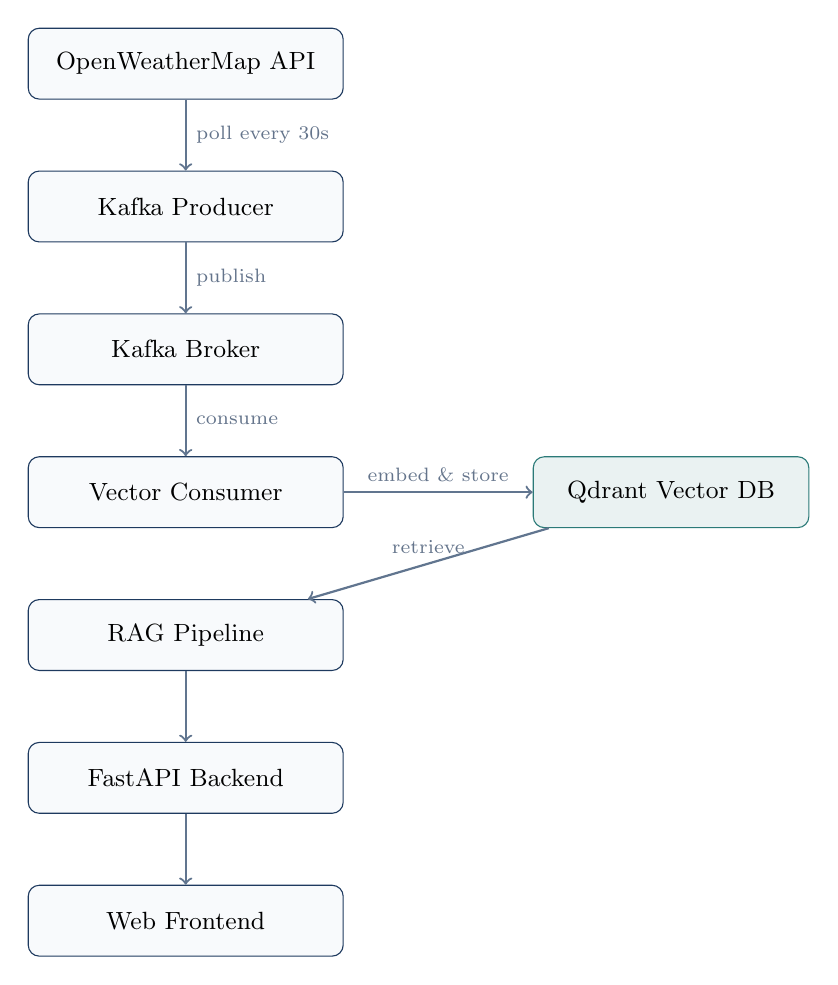
\begin{tikzpicture}[
    node distance=0.9cm,
    box/.style={draw=primary, fill=lightbg, rounded corners=4pt, minimum width=4cm, minimum height=0.9cm, text centered, font=\small},
    dbbox/.style={draw=secondary, fill=secondary!10, rounded corners=4pt, minimum width=3.5cm, minimum height=0.9cm, text centered, font=\small},
    arrow/.style={->, thick, primary!70},
    label/.style={font=\scriptsize, color=textmuted}
]
    \node[box] (api) {OpenWeatherMap API};
    \node[box, below=of api] (producer) {Kafka Producer};
    \node[box, below=of producer] (kafka) {Kafka Broker};
    \node[box, below=of kafka] (consumer) {Vector Consumer};
    \node[dbbox, right=of consumer, xshift=1.5cm] (qdrant) {Qdrant Vector DB};
    \node[box, below=of consumer] (rag) {RAG Pipeline};
    \node[box, below=of rag] (fastapi) {FastAPI Backend};
    \node[box, below=of fastapi] (frontend) {Web Frontend};
    
    \draw[arrow] (api) -- (producer) node[midway, right, label] {poll every 30s};
    \draw[arrow] (producer) -- (kafka) node[midway, right, label] {publish};
    \draw[arrow] (kafka) -- (consumer) node[midway, right, label] {consume};
    \draw[arrow] (consumer) -- (qdrant) node[midway, above, label] {embed \& store};
    \draw[arrow] (qdrant) -- (rag) node[midway, above, label] {retrieve};
    \draw[arrow] (rag) -- (fastapi);
    \draw[arrow] (fastapi) -- (frontend);
\end{tikzpicture}
\caption{System architecture showing data flow from API ingestion through streaming, storage, and presentation layers.}
\label{fig:architecture}
\end{figure}

\subsection{Data Ingestion Layer}

The Kafka producer runs as a continuous background process, polling the OpenWeatherMap API on a configurable interval (default 120 seconds). Each API response undergoes enrichment with:
\begin{itemize}[leftmargin=2em, itemsep=0.1em]
    \item \texttt{location} field for geographic filtering
    \item \texttt{ingestion\_time} timestamp for temporal analysis
    \item \texttt{data\_type} classification for routing
\end{itemize}

\subsection{Stream Processing Layer}

The vector consumer performs three operations for each message:
\begin{enumerate}[leftmargin=2em, itemsep=0.2em]
    \item \textbf{Text Generation} -- Construct natural language from structured JSON
    \item \textbf{Embedding} -- Generate 384-dimensional vectors via multilingual sentence transformer
    \item \textbf{Storage} -- Upsert to Qdrant with metadata payload
\end{enumerate}

\subsection{News Integration}

StormWatch AI ingests French weather news via RSS feeds from Le Monde's climate section, filtering articles by keywords: \textit{vigilance}, \textit{tempête}, \textit{inondation}.

\newpage
%% ========================================
\section{Application Interface}
%% ========================================

The web application provides an intuitive interface for weather queries. Figure~\ref{fig:screenshot} shows the main interface.

\begin{figure}[H]
\centering
\fbox{\includegraphics[width=0.85\textwidth]{screenshot.png}}
\caption{StormWatch AI web interface: sidebar with current conditions (left) and chat area for natural language queries (right).}
\label{fig:screenshot}
\end{figure}

\subsection{Interface Components}

\begin{table}[H]
\centering
\caption{Web interface components}
\renewcommand{\arraystretch}{1.3}
\begin{tabular}{l p{10cm}}
\toprule
\textbf{Component} & \textbf{Features} \\
\midrule
Sidebar & City selector, 2×2 metrics grid (temperature, humidity, wind, conditions), alerts section, ``Live Data'' status badge \\
Chat Area & Quick-action buttons, custom query input, user/AI message styling with markdown \\
Header & StormWatch AI branding, assistant description \\
\bottomrule
\end{tabular}
\end{table}

A critical design decision ensures consistency: all weather data in the sidebar originates from Qdrant, not direct API calls. This ensures that when users ask follow-up questions, the RAG system retrieves the same underlying data they see displayed.

\newpage
%% ========================================
\section{Implementation Details}
%% ========================================

\subsection{Embedding Model Selection: Cross-Lingual News Retrieval}

The system initially used \texttt{all-MiniLM-L6-v2}, an English-optimized sentence transformer. However, StormWatch AI ingests French news from Le Monde RSS feeds, requiring users to query French content with potentially English questions. Since weather data retrieval is deterministic (filter by city/timestamp), only news article retrieval uses semantic RAG, making cross-lingual embedding quality critical.

\subsubsection{Benchmark Methodology}

We constructed a test set pairing \textbf{English user queries} with \textbf{French news excerpts} from Le Monde's climate RSS feed. For each pair, we embedded both texts and computed cosine similarity. Table~\ref{tab:test-pairs} shows the complete test set.

\begin{table}[H]
\centering
\caption{Test query-article pairs for cross-lingual news retrieval evaluation}
\label{tab:test-pairs}
\renewcommand{\arraystretch}{1.25}
\small
\begin{tabular}{p{5.5cm} p{7.5cm}}
\toprule
\textbf{English Query} & \textbf{French Article Excerpt (Le Monde)} \\
\midrule
What are the cold weather protection measures? & Plan Grand Froid : plusieurs préfectures ont actionné des mesures d'urgence pour protéger les plus vulnérables. \\
What emergency actions have been taken by the government? & Face à la vague hivernale, la Mairie de Paris réclame le déclenchement du plan Grand Froid, l'État répond être largement mobilisé. \\
Is there a flood warning in the region? & Pluie-inondation : la vigilance orange maintenue dans les Pyrénées-Orientales avec des cumuls de 30 à 50 mm. \\
Are there any storm warnings? & Pluie-inondations : la vigilance orange levée en Haute-Corse ; les Pyrénées-Orientales maintenues en alerte. \\
Will it snow tomorrow? & Neige en France : deux départements en vigilance orange, des chutes de 5 à 10 cm localement. \\
How strong is the wind today? & Vents violents attendus sur la côte atlantique avec des rafales jusqu'à 100 km/h selon Météo-France. \\
\bottomrule
\end{tabular}
\end{table}

\subsubsection{Cross-Lingual Retrieval Results}

\begin{table}[H]
\centering
\caption{Cross-lingual similarity scores (EN query $\rightarrow$ FR article)}
\renewcommand{\arraystretch}{1.2}
\begin{tabular}{l c c c}
\toprule
\textbf{Query Topic} & \textbf{MiniLM (EN)} & \textbf{Multilingual} & \textbf{Improvement} \\
\midrule
Cold weather measures & 0.18 & \textbf{0.70} & +288\% \\
Emergency actions & 0.21 & \textbf{0.40} & +92\% \\
Flood warning & 0.18 & \textbf{0.55} & +213\% \\
Storm warnings & 0.31 & \textbf{0.44} & +40\% \\
Snow forecast & 0.02 & \textbf{0.12} & +572\% \\
Wind conditions & 0.15 & \textbf{0.50} & +229\% \\
\midrule
\textbf{Average} & \textbf{0.17} & \textbf{0.45} & \textbf{+159\%} \\
\bottomrule
\end{tabular}
\end{table}

The multilingual model nearly \textbf{triples} cross-lingual similarity scores (0.17 $\rightarrow$ 0.45). This improvement is critical for news retrieval: scores below 0.3 typically fail to surface relevant articles, while scores above 0.4 reliably match user intent.

\subsubsection{Trade-off Analysis}

The multilingual model introduces a 27\% speed penalty (4,648 vs 6,363 sentences/second). However, both exceed real-time requirements. The cross-lingual gains justify this trade-off for bilingual news retrieval.

\begin{highlightbox}[Design Decision]
StormWatch AI uses \texttt{paraphrase-multilingual-MiniLM-L12-v2} to enable cross-lingual queries, accepting a minor speed trade-off for 2$\times$ improved retrieval of French weather news.
\end{highlightbox}

\subsection{Type-Specific Retrieval Strategies}

StormWatch AI uses different retrieval strategies depending on data type. Weather data (current conditions, forecasts, air quality) is retrieved \textbf{deterministically} using filters and timestamp sorting. Only news articles use \textbf{semantic RAG with temporal decay}.

\subsubsection{Deterministic Retrieval (Weather Data)}

Weather data has a known structure and freshness requirement. Retrieval uses Qdrant's payload filtering without semantic search:

\begin{table}[H]
\centering
\caption{Deterministic retrieval methods for structured weather data}
\renewcommand{\arraystretch}{1.3}
\begin{tabular}{l p{9cm}}
\toprule
\textbf{Data Type} & \textbf{Retrieval Method} \\
\midrule
Current Weather & Filter by \texttt{data\_type="current\_weather"} and \texttt{location}, sort by timestamp descending, return newest entry \\
Air Quality & Filter by \texttt{data\_type="air\_quality"} and \texttt{location}, sort by timestamp descending, return newest entry \\
Forecast & Filter by \texttt{data\_type="forecast"} and \texttt{location}, sort by timestamp descending, return 2-3 newest entries \\
Alerts & Filter by \texttt{data\_type="alert"}, return entries where \texttt{start} $\leq$ now $\leq$ \texttt{end} \\
\bottomrule
\end{tabular}
\end{table}

\subsubsection{Semantic RAG with Temporal Decay (News Articles)}

News retrieval is the only component using true RAG: it combines \textbf{semantic similarity} (via embedding cosine distance) with \textbf{temporal decay} to prioritize both relevance and freshness.

\begin{enumerate}[leftmargin=2em, itemsep=0.2em]
    \item \textbf{Embed the user query} using the multilingual sentence transformer
    \item \textbf{Vector search} in Qdrant filtered by \texttt{data\_type="news"}
    \item \textbf{Apply time decay} to re-rank by freshness:
\end{enumerate}

\begin{mathbox}
\[
s_{\text{final}} = s_{\text{similarity}} \cdot e^{-t / 24}
\]

\vspace{0.3em}
\small
where $t$ = article age in hours. Decay rate: 50\% retention after 24 hours.
\end{mathbox}

\begin{table}[H]
\centering
\caption{News score retention over time}
\renewcommand{\arraystretch}{1.2}
\begin{tabular}{cc}
\toprule
\textbf{Article Age} & \textbf{Score Retention} \\
\midrule
1 hour & 95.9\% \\
6 hours & 77.9\% \\
12 hours & 60.7\% \\
24 hours & 36.8\% \\
\bottomrule
\end{tabular}
\end{table}

This ensures today's ``Plan Grand Froid'' article ranks higher than last week's weather news, even if both are semantically similar to the query.

\subsection{Location Filtering with Payload Indexes}

Qdrant implements efficient filtering via \textbf{payload indexes} (B-tree structures on metadata fields):

\begin{lstlisting}[language=Python]
client.create_payload_index(
    collection_name="weather_data",
    field_name="location",
    field_schema=PayloadSchemaType.KEYWORD
)
\end{lstlisting}

This enables two-phase search: (1) prune to matching payload values, (2) vector similarity within filtered subset. Query latencies remain sub-100ms even as collection grows.

\newpage
%% ========================================
\section{Conclusion}
%% ========================================

This report presented \textbf{StormWatch AI}, a real-time weather advisory system that integrates Apache Kafka for stream processing, Qdrant for vector storage, and retrieval-augmented generation with Groq LLM inference.

A central design choice was \textbf{differentiated retrieval}: rather than applying uniform RAG to all data types, the system uses database-style filtering for structured weather data, validity-period checking for alerts, and semantic search with temporal decay exclusively for news articles. This approach matches retrieval methods to data characteristics, ensuring both accuracy and efficiency.

The architecture combining Kafka, vector databases, and RAG represents a reusable pattern for domains requiring conversational access to streaming data, such as financial news analysis, IoT sensor monitoring, and real-time event tracking.

A potential extension would be to leverage LLM tool-use capabilities, where the model dynamically generates Qdrant queries based on user intent. This would increase flexibility but adds latency and complexity; our explicit retrieval logic prioritizes reliability and speed for the well-defined weather domain.

\newpage
%% ========================================
%% BIBLIOGRAPHY
%% ========================================

\begin{thebibliography}{9}

\bibitem{kafka}
Kreps, J., Narkhede, N., and Rao, J. (2011). Kafka: A distributed messaging system for log processing. \textit{Proceedings of the NetDB Workshop at SIGMOD}.

\bibitem{qdrant}
Qdrant Team. (2024). Qdrant: Vector similarity search engine with extended filtering support. \url{https://qdrant.tech/}

\bibitem{rag}
Lewis, P., et al. (2020). Retrieval-augmented generation for knowledge-intensive NLP tasks. \textit{Advances in Neural Information Processing Systems}, 33, 9459--9474.

\bibitem{openweather}
OpenWeatherMap. (2024). Weather API documentation. \url{https://openweathermap.org/api}

\bibitem{groq}
Groq Inc. (2024). Groq LPU Inference Engine. \url{https://groq.com/}

\bibitem{sbert}
Reimers, N. and Gurevych, I. (2019). Sentence-BERT: Sentence embeddings using Siamese BERT-networks. \textit{Proceedings of EMNLP 2019}, 3982--3992.

\end{thebibliography}

\end{document}
